
\documentclass[conference]{IEEEtran}
\IEEEoverridecommandlockouts
\renewcommand{\baselinestretch}{1.5}
\usepackage{cite}
\usepackage{amsmath,amssymb,amsfonts}
\usepackage{algorithmic}
\usepackage{graphicx}
\usepackage{textcomp}
\usepackage{xcolor}
\def\BibTeX{{\rm B\kern-.05em{\sc i\kern-.025em b}\kern-.08em
    T\kern-.1667em\lower.7ex\hbox{E}\kern-.125emX}}
\begin{document}


\title{Análisis en SPSS sobre la influencia de diferentes factores en la felicidad de los estudiantes de la Universidad Distrital Francisco José de Caldas
(marzo de 2020)
}

\author{\IEEEauthorblockN{1\textsuperscript{st} Alvaro Alejandro Zarabanda Gutierrez. }
\IEEEauthorblockA{\textit{aazarabandag@correo.udistrital.edu.co,}}
\and
\IEEEauthorblockN{2\textsuperscript{nd}  Raúl Eduardo Pachón Alarcón. }
\IEEEauthorblockA{\textit{repachona@correo.udistrital.edu.co,}}}

\maketitle

\textbf{\textit{Resumen--}
Se busca determinar el comportamiento de la felicidad de los estudiantes en función de variables que, con base en otros estudios y sentido común, son influyentes en esta. Puesto que en los últimos años en la universidad la tasa de deserción ha aumentado, haciendo uso de una encuesta que incluye como sub encuesta The Oxford Happiness Questionnaire para hallar el índice de felicidad y complementando con otra sub encuesta experimental basada en las variables encontradas, se desea encontrar cuales de estas variables son realmente influyentes en la felicidad de los estudiantes. Utilizando como herramienta el software SPSS (Statistical Package for the Social Sciences), como primer paso se pretende comprobar la fiabilidad de ambas sub encuestas, donde se corrobora el alto coeficiente de fiabilidad de la primera, y se hace un detenido análisis sobre la segunda, esto debido a su bajo coeficiente de fiabilidad. Como segundo paso, se aplica el modelo de Regresión Logística Binaria para lograr el objetivo ya mencionado, donde variables como “Es creyente” y “Estado Civil” arrojan resultado positivo en cuanto a significancia, no obstante, se tiene en cuenta que estos hallazgos pueden ser solo aplicables a un pequeño porcentaje de la población, ya que estos son totalmente dependientes de la fiabilidad.\\\\
Índice de Términos – Análisis, Correlación, Covarianza, Encuesta, Escala, Ecuación, Fiabilidad, Felicidad, Matriz, Probabilidad, Programa, Regresión, Satisfacción Personal, Variable.\\}

\section{INTRODUCCIÓN}\\


\IEEEPARstart{E}{\\}l concepto de felicidad ha desconcertado al ser humano a lo largo de su existencia como especie. Por lo que ha desarrollado una gran variedad de definiciones e investigaciones en torno a este concepto. Estas definiciones han tenido diversos factores sobre los cuales se soportan. Debido a la variación de los parámetros empleados para el desarrollo de estas investigaciones se han precisado algunas perspectivas como: Alarcón [1], basado en la filosofía griega y los recientes estudios, la define como: “un estado de satisfacción, más o menos duradero, que experimenta subjetivamente el individuo en posesión de un bien deseado”, también se han generado perspectivas opuestas como: Fernández D. [2] propone que los factores que influyen en la felicidad, radican en nuestro interior y poco tiene que ver con la acumulación de bienes.\\

   Si bien es debatible que la vida universitaria es uno de los estilos de vida más estresantes, se sabe que hay muchos casos donde los estudiantes universitarios dicen sentirse estresados o presionados por diferentes factores tales como lo son realización de exámenes, trabajos individuales y grupales, practicas, fechas de entrega, establecimiento de relaciones sociales, etc. [3] Muchas veces al buscar una alternativa para vencer el estrés se tiene el consumo de alcohol, el cual tiene como “beneficio” la aceptación y un mejor ajuste psicosocial [4], sin embargo también está la caída de rendimiento académico debido a su abuso, lo cual conlleva a posibles estados de depresión y problemas de salud. [5]\\

   Como se puede observar, la felicidad es un caso de estudio que tiene investigaciones desde una perspectiva muy general hasta una bastante específica, no obstante, esta tendrá un mayor enfoque hacia la satisfacción del estudiante, donde se estará en una constante búsqueda de lograr una educación orientada hacia la felicidad del estudiante, para que análogamente se logre una disminución en la tasa de deserción que hay actualmente.\\



\section{METODOLOGÍA}\\
\subsection{Diseño}\\
   Este es un diseño correlacional experimental, que se quiere implementar y mejorar paulatinamente para poder encontrar que tipo de comportamientos son los que más relacionados están con la felicidad de los estudiantes. Para esto se toma como base la encuesta: The Oxford Happiness Questionnaire desarrollada por los psicólogos Michael Argyle y Peter Hills [6] y la encuesta experimental de las variables independientes que contiene los siguientes ítems:\\
   
   
   \begin{itemize}
    \item Edad\item Género \item Semestre \item Estrato económico \item Estado civil \item Trabaja\item ¿EL nivel de sus ingresos con respecto a sus gastos mensuales son?	 \item Promedio académico \item Es creyente \item ¿Quién costea sus estudios? \item Tiempo promedio
    diario de uso del celular \item ¿En que tipo de casa vive? \item Tiempo de desplazamiento casa-universidad\\
\end{itemize}\
      Donde todas sus respuestas son de carácter dicótomo. No se tomó en cuenta ningún tipo de clasificación grupal para la toma de las muestras, debido a que como primer paso se quiere hacer una generalización.
   
\subsection{Muestra}\\	

   Para este caso de estudio, se tomó una muestra de 302 estudiantes de pregrado de la Universidad Distrital pertenecientes a cualquiera de las facultades. La estrategia de muestreo fue aleatorio simple, donde el llenado de la encuesta fue totalmente voluntario.\\

\subsection{Materiales}\\

   El cuestionario empleado en el desarrollo del presente trabajo consto de un total de 42 preguntas de las cuales 29 pertenecen a The Oxford Happiness Questionnaire [6]. Estas 29 preguntas tienen un tipo de respuesta denominada escala Likert. Mientras que las 13 peguntas restantes son aquellas que ya se mencionaron en el diseño.\\



\begin{table}[h]
\caption{Escala Tipo Likert The Oxford Happiness Questionnaire}
\label{tabla 1}
\begin{center}
\begin{tabular}{|c||c|}
\hline
Totalmente en desacuerdo & 1\\ \hline
Más o menos en desacuerdo & 2\\ \hline
Ligeramente en desacuerdo & 3\\ \hline
Ligeramente en acuerdo & 4\\ \hline
Más o Menos de acuerdo & 5\\ \hline
Totalmente de acuerdo & 6\\ \hline
\end{tabular}
\end{center}
\end{table}\\
   Sin embargo, La esta escala original mostrada en la tabla 1 fue modificada de 6 categorías a 5 como se aprecia en la tabla 2, debido a que la escala de Likert más común contiene 5 categorías y de acuerdo a un análisis interno realizado con anterioridad no se encontró significancia suficiente para manejar dichas categorías.\\
   
   \begin{table}[h]
\caption{TRANSFORMACION ESCALA TIPO LIKERT THE OXFORD HAPPINESS QUESTIONNAIRE}
\label{tabla 1}
\begin{center}
\resizebox{8.8cm}{!} {
\begin{tabular}{|c||c||c|}
\hline
valor original & nuevo valor & valor numérico \\
\hline \hline \hline
Totalmente en desacuerdo & Totalmente en desacuerdo & 1\\ \hline
Más o menos en desacuerdo & Más o menos en desacuerdo & 2\\ \hline
Ligeramente en desacuerdo & Ni en acuerdo ni desacuerdo & 3\\ \hline
Ligeramente en acuerdo &Ni en acuerdo ni desacuerdo & 3\\ \hline
Más o Menos de acuerdo & Más o Menos de acuerdo & 4\\ \hline
Totalmente de acuerdo & Totalmente de acuerdo & 5\\ \hline
\end{tabular}
}
\end{center}
\end{table}
   Como herramienta principal se usó el software SPSS (Statistical Package for the Social Sciences), el cual es un programa destinado al análisis de datos ofrecido por IBM. Este contiene todas las herramientas necesarias para llevar a cabo completos estudios estadísticos. Gracias a él es posible realizar recopilación de datos, crear estadísticas, análisis de decisiones de gestión y manejo de gráficos de datos obtenidos\\               

   Esta nos ofrece una manera sencilla de hacer los análisis introduciendo la serie de datos que tenemos de la encuesta, y con una secuencia paso a paso podemos aplicar fácilmente los modelos matemáticos para hacer los análisis de fiabilidad y regresión. \\  

   También se hará uso de estadísticos descriptivos en el software para obtener un panorama más general acerca de los resultados.\\

\subsection{Procedimiento}
   Para el posterior tratamiento de los datos obtenidos en la encuesta se aplica el procedimiento realizado en la encuesta de Oxford, con la finalidad de determinar el valor que tendrá nuestra variable dependiente en cada uno de los registros. Este valor se determina hallando el promedio de las respuestas dadas en el cuestionario este resultado en el trabajo de Oxford es un número entre 1 y 6 sin embargo teniendo en cuenta el cambio en la escala de Likert realizada el resultado en este caso será un numero entre 1 y 5. En cuanto al valor que se debe asignar a la variable principal, para el tipo de análisis que se desea aplicar, es dicótomo, por lo que se decidió hallar el promedio de las calificaciones de todos los encuestados y utilizar ese valor como punto de quiebre entre los dos respuestas “Es Feliz” y “No es Feliz”.\\
   \begin{table}[h]
\caption{Escala Tipo Likert }
\label{tabla 1}
\begin{center}
\begin{tabular}{|c||c||c|}
\hline
 Totalmente en desacuerdo & 1\\ \hline
 Más o menos en desacuerdo & 2\\ \hline
 Ni en acuerdo ni desacuerdo & 3\\ \hline
 Más o Menos de acuerdo & 4\\ \hline
 Totalmente de acuerdo & 5\\ \hline
\end{tabular}
\end{center}
\end{table}
   Se tiene la versión 25 del software SPSS, donde se procede a hacer la importación de los datos que se obtienen de la encuesta que están en formato CSV, luego de eso en la pestaña analizar tenemos diferentes opciones, donde una de ellas es el análisis de fiabilidad. Para el caso de la encuesta de Oxford, solo se deben seleccionar las 29 preguntas que hacen parte de esta, luego, haciendo el mismo procedimiento, se hace el análisis de fiabilidad, pero en este caso solamente de las variables independientes.\\

   Por otro lado, con la regresión logística binaria, se accede al apartado que dice regresión que está en la pestaña ya mencionada, allí se selecciona regresión logística binaria y se mostrara una nueva ventana donde se debe introducir la variable dependiente y las variables independientes, finalmente se debe finalizar el procedimiento para obtener las tablas de los resultados.\\

\section{Resultados}\\
 En términos generales, podemos observar el comportamiento de los encuestados en cuanto a la encuesta de Oxford haciendo uso de simples estadísticos descriptivos, donde podemos observar: \\
 \begin{center}
\caption{TABLE IV\\
ESTADISTICOS DESCRIPTIVOS}
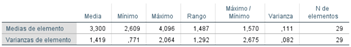
\includegraphics[width=8.5cm]{imagenes/tabla5.png}
\end{center}
La media sobrepasa la mitad de la calificación de la escala tipo Likert propuesta del OHQ, la cual es 2.5. Esto nos da un indicio de que la gran mayoría de los estudiantes de la universidad posiblemente se podrían clasificar como que no son particularmente felices o infelices según los resultados de la escala, sin embargo, se debe tomar en cuenta la dispersión que tienen los datos, puesto que podemos observar la varianza que se obtiene, y el dato mínimo y máximo con respecto a la media, por lo que con el uso de estos estadísticos no podríamos obtener resultados fiables en la investigación.\\
\begin{center}
\caption{TABLE V\\
COEFICIENTE ALFA DE CRONBACH OHQ}
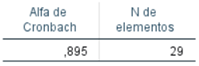
\includegraphics[width=7cm]{imagenes/tabla51.png}
\end{center}
Coeficiente alfa de Cronbach.  En la primera columna de la tabla 5, podemos observar el coeficiente Alfa de Cronbach total del instrumento, el cual fue de 0.895, lo cual es aceptable teniendo en cuenta que el mínimo confiable es de 0.7. Esto significa que se cumple la tendencia o resultados esperados, donde la consistencia de la encuesta es alta basada en otros estudios como el de Alarcón, Reynaldo [1] o  K.E. Gamero Tafur, E.M. Medina Martínez, A. Escobar Espinoza [11], donde también se corrobora la fiabilidad del OHQ.\\
\begin{center}
\caption{TABLE VI\\
COEFICIENTE DE FIABILIDAD ENCUESTA EXPERIMENTAL}

\includegraphics[width=7cm]{imagenes/IMAGEN15.png}
\end{center}
Análisis de fiabilidad KR-20. Para las variables independientes, se hizo uso de este coeficiente de fiabilidad, eso teniendo en cuenta que son variables dicótomas. Para hacer este procedimiento en SPSS es de la misma manera a como se hizo con el alfa de Cronbach, y en la columna 1 de la tabla 6 observamos que es muy bajo el coeficiente de fiabilidad. Esto nos dice que no es muy buena practica aplicar encuestas experimentales, sien embargo como este es un método de consistencia de encuestas correlacional [9], puede haber una manera de aumentar la consistencia eliminando uno o varios elementos dependiendo de los resultados.\\

\begin{center}
\caption{TABLE VI\\
CONSISTENCIA DE ENCUESTA EXPERIMENTAL SI SE SUPRIMEN ELEMENTOS
}
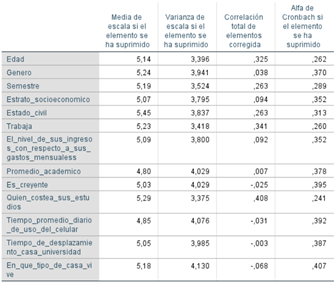
\includegraphics{imagenes/tabla6.png}
\end{center}
 Como podemos observar en la tabla 6 en la columna 5, la consistencia de la encuesta puede ir aumentando significativamente. La idea de la consistencia es que los elementos de la encuesta no estén correlacionados positivamente o que su correlación sea inversa o cercana a 0, lo que es básicamente la homogeneidad del cuestionario. [9] \\
   
   Regresión logística binaria. Esta no arroja resultados muy alentadores debido a lo que pudimos observar con la fiabilidad de la encuesta experimental, y esto también lo podemos corroborar con los R$^2$  de Cox y Snell y R$^2$ de Nagelkerke (ver taba 7), donde sus coeficientes nos indican en que medida las variables independientes explican la variable dependiente [12], para nuestro caso de estudio, se obtuvieron coeficientes muy bajos.\\
\begin{center}
\caption{TABLE VII\\
RESUMEN DEL MODELO}
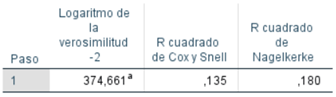
\includegraphics{imagenes/IMAGEN21.png}
\end{center}
\begin{center}
\caption{TABLE VIII\\
CLASIFICACION}
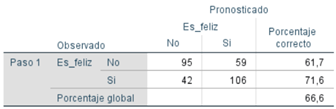
\includegraphics{imagenes/IMAGEN23.png}
\end{center}
  No obstante, se terminó de aplicar el modelo de Regresión para obtener las variables independientes significativas del modelo.\\

  En la columna 1 de la tabla 9, podemos observar las variables independientes y en la columna 6 podemos ver su significancia. Un resultado es estadísticamente significativo si se corresponde con un valor p igual o inferior al nivel de significación, es decir, para este caso un valor p ≤ 0.05 [13]\\
\begin{center}
\caption{TABLE IX\\
VARIABLES EN EL MODELO DE REGRESION}
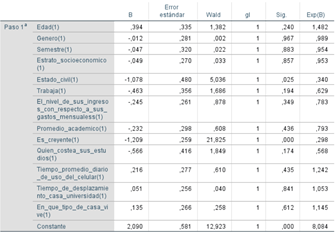
\includegraphics{imagenes/IMAGEN24.png}
\end{center}
Al terminar de realizar la regresión logística binaria, se obtuvo como variables significativas “Estado Civil” y “Es creyente” con un p valor o significancia de 0.025 y 0.000 respectivamente, donde el modelo explica de un 13\% a un 18\% la variable felicidad con respecto a las variables independientes [12] y clasifica correctamente el 66.6\% de los casos. [13] (Ver tabla 8)\\

Ahora teniendo las variables significativas, se puede aplicar la ecuación logística [10] para construir el modelo predictivo.\\

\textbf{Teniendo esta información, primero aplicaremos la ecuación general en la variable “Es creyente” donde la categoría de referencia es No=1 y Felicidad Si=1, ya que de esta manera quedo codificado en el programa SPSS. Entonces la ecuación sería:}\\
\begin{equation}\tiny
P\left(FELICIDAD=SI\right)=\frac{1}{\left(1+e^{\left(\left(-2.090-\left(-1.209\cdot \:"ES\:CREYENTE"\right)\right)\:\right)}\right)}
\end{equation}
   Ahora, se calculará reemplazando el valor ES CREYENTE=1, donde 1=No (Cat. de referencia). \\
   \begin{equation}\tiny
 P\left(FELICIDAD=SI\right)=\frac{1}{\left(1+e^{\left(\left(-2.090-\left(-1.209\cdot \:1\right)\right)\:\right)}\right)}=0.7070
 \end{equation}
Esto lo podemos interpretar, que con esta probabilidad predicha mayor a 0.50 una persona no creyente se clasificaría como FELICIDAD=SI. Cabe recalcar que hay otros factores que influyen en este resultado como lo son el porcentaje correcto de clasificación arrojado por el modelo (Ver tabla 8) y el coeficiente de fiabilidad (Ver tabla 6).\\

\textbf{A continuación, se hará el análisis con la variable “Estado civil” donde, de la misma manera la categoría de referencia es Soltero=1 y Felicidad Si=1.}\\   
\begin{equation}\tiny
P\left(FELICIDAD=SI\right)=\frac{1}{\left(1+e^{\left(\left(-2.090-\left(-1.209\cdot \:"ESTADO\:CIVIL"\right)\right)\:\right)}\right)}
\end{equation}
   Ahora, se calculará reemplazando el valor ES CREYENTE=1, donde 1=No (Cat. de referencia). \\
   \begin{equation}\tiny
 P\left(FELICIDAD=SI\right)=\frac{1}{\left(1+e^{\left(\left(-2.090-\left(-1.078\cdot \:1\right)\right)\:\right)}\right)}=0.7334
 \end{equation}
 Esto lo podemos interpretar, que con esta probabilidad predicha mayor a 0.50 una persona soltera se clasificaría como FELICIDAD=SI.\\
\section{Conclusiones}
  
  Los datos obtenidos del desarrollo de este trabajo   indican que tanto la herramienta de recolección (encuesta) como los resultados son confiables en cuanto a las preguntas obtenidas de Oxford Happiness Questionnaire, de esta manera se valida la efectividad de este cuestionario. Para las preguntas incluidas en la encuesta desarrollada se empleó el análisis KR- 20 y la regresión logística binaria para determinar cuáles de las variables propuestas realmente tenían una relación directa con la felicidad. En este proceso se determinó como variables significativas “Es creyente” y “Estado civil”, en donde estas explican el modelo de manera correcta entre un 13\% y un 18\%. por lo cual es necesario encontrar más variables para predecir la variable principal de una manera más completa y exacta. Para la primera variable encontrada se determinó que su valor se relaciona de manera directamente proporcional con la variable principal cuando su valor es “no creyente”, mientras que el valor de estado civil es directamente proporcional respecto a la variable principal cuando las personas son solteras. Por lo tanto, se obtiene que dentro del aglomerado estudiantil de la Universidad Distrital Francisco José de Caldas las dos características anteriormente mencionadas parcialmente a las personas identificadas como felices.\\\
 
\section{DISCUSION}\\

A pesar de no poder obtener resultados contundentes, se puede comprobar la tendencia de que las variables “Es creyente” y “Estado civil” son significativas en el momento de predecir la felicidad en determinado grupo estudiado, como lo es en este caso en estudiantes universitarios. En base al caso de estudio de  Gamero Tafur, Medina Martínez y Escobar Espinoza [7] podemos evidenciar que estas variables también jugaron un papel importante en su investigación, sin embargo cabe aclarar que las probabilidades que ellos obtuvieron fueron totalmente distintas a las de este estudio, puesto que como ejemplo en la variable “Estado Civil”, en este estudio se obtiene mayor probabilidad de predicción de 73.34\% de que una persona sea feliz cuando esta soltera, caso contrario al del estudio referenciado, donde el matrimonio es significativo e importante debido a las satisfacciones que genera la confianza y el intercambio de confidencias y opiniones entre esta cooperativa [8], no obstante podemos tener en cuenta que hablar de matrimonio es un caso en el cual la edad promedio de la realización de este es entre los 28 y 32 años [9] y considerando que más del 50\% de los encuestados son menores de 20 años, hablar de matrimonio puede ser no muy coherente, puesto que muchos jóvenes de hoy en día piensan diferente en cuanto a la vida en pareja. Eliakim Kislev [10], afirma que los solteros cuentan con un mayor poder de sentir felicidad y satisfacción, por ende, son menos egoístas a diferencia de aquellos que llevan una vida en pareja.

   Un soltero regularmente, no quiere decir que así sea en todos los casos, experimenta mayor libertad, ya que no tiene que llegar a acuerdos con alguien más durante la toma de decisiones. Los solteros se sienten más completos en su profesión, vida diaria, vida social y más, sobre todo con mayor libertad para hacer planes [10], y con esto viene conjunto otras configuraciones de pareja  como “amigos con derecho”, “amigovios”, “parche”, “relaciones sexuales”, “relaciones virtuales”, frente a relaciones con compromiso, amor, confianza y construcción de intimidad [11] que actualmente muchos jóvenes practican, con esto podemos decir de forma más general que la felicidad en función de la variable estado civil es totalmente dependiente del grupo de edades estudiado, por otro lado, podemos observar la investigación hecha por Macaya Sazo, Marlene Fernandan [12], en el cual la muestra fue de hombres y mujeres de un rango de edad entre 18 y 30 y donde se concluye que las variables que se relacionan con aspectos relacionales o afectivos, son las que explican en su mayoría el nivel de felicidad de estos estudiantes, con lo que podemos afirmar que esta variable siempre se debe incluir en futuros estudios.

   En cuanto a la variable “Es creyente”  tomando de nuevo como base la investigación hecha por Gamero Tafur, Medina Martínez, Escobar Espinoza [7], se muestra que esta tiene una discrepancia en el modelo explicativo de la felicidad, esta información revela una  diferencia existente entre la percepción de la religión entre las  distintas poblaciones, pues en este estudio, se evidencia que las personas no creyentes o dicho de otra manera, no practicantes de alguna religión tienen mayor probabilidad de ser felices y teniendo en cuenta una encuesta una encuesta internacional realizada por la empresa Gallup [13] hecha entre 2005 y 2011 revela que el número de personas que se consideran religiosas disminuyo de un 77\% a un 68\% y esto lo tenemos como una tendencia que va en aumento con el tiempo.




\begin{thebibliography}{99}
\bibitem{c1} R. Alarcon, «Desarrollo de una escala factorial para medir la felicidad,» Interamerican Journal of Psychology, 2006, pp. 95-102.
\bibitem{c2}	M. R. F. Fernández D., Construyendo nuestra felicidad para ayudar a construirla, 2009, pp. 231-239.
\bibitem{c3}	H. Figueiredo-Ferraz, S. Cardona y P. Gil Monte, «Desgaste psíquico y problemas de salud en estudiantes de psicologia,» Psicologia em Estudo, 2009. 
\bibitem{c4}	M. Newcomb y P. Bentler, «Impact of adolescent drug use and social support on problems of young adults: A longitufinal study,» Journal of Abnormal, pp. 64-75, 1988. 
\bibitem{c5}	S. Casswell, Ru Quan You y H. Taisia, «Alcohol's harm to others:Reduced wellbeing and health status for those with heavy drinkers in their lives,» Addiction, pp. 1087-1094, 2011. 
\bibitem{c6}	M. Argyle y P. Hills, Oxford Happiness Questionnaire, 2008. 
\bibitem{c7}	K. E. G. Tafur, E. M. M. Martínez y A. A. E. Espinoza, La felicidad en estudiantes universitarios de ciencias económicas: algunos determinantes socioeconómicos en la ciudad de Cartagena de Indias, 2017. 
\bibitem{c8}	M. Argyle, «Causes and correlates of happiness,» Well-Being: The foundations of hedonic psychology, pp. 353-373, 1999. 
\bibitem{c9}	COLPRENSA, «El Universal,» 9 Agosto 2015. [En línea]. Available: https://www.eluniversal.com.co/salud/cual-es-la-edad-ideal-para-casarse-202252-ATEU303506.
\bibitem{c10}	E. Kislev, Happy Singlehood: The Rising Acceptance and Celebration of Solo Living. 
\bibitem{c11}	A. I. Blandon Hincapie y L. M. Lopez Serna, «Comprensiones sobre pareja en la actualidad: Jovenes en busca de la estabilidad,» Revista Latinoamericana de Ciencias Sociales, Niñez y Juventud, pp. 505-517, 2016. 
\bibitem{c12}	M. F. Macaya Sazo, «Nivel de felicidad en estudiantes universitarios de la comuna de Talca,» 2015. 
\bibitem{c13}	Gallup Corporation, «Gallup,» 2005. [En línea]. Available: https://www.gallup.com/es-xm/176819/gallup-latin-america.aspx.









\end{thebibliography}

\end{document}




